\documentclass{standalone}
\usepackage{tikz}
\usetikzlibrary{positioning}
\usetikzlibrary{shadows}
\usetikzlibrary{shapes}
\usepackage{graphicx}
\begin{document}
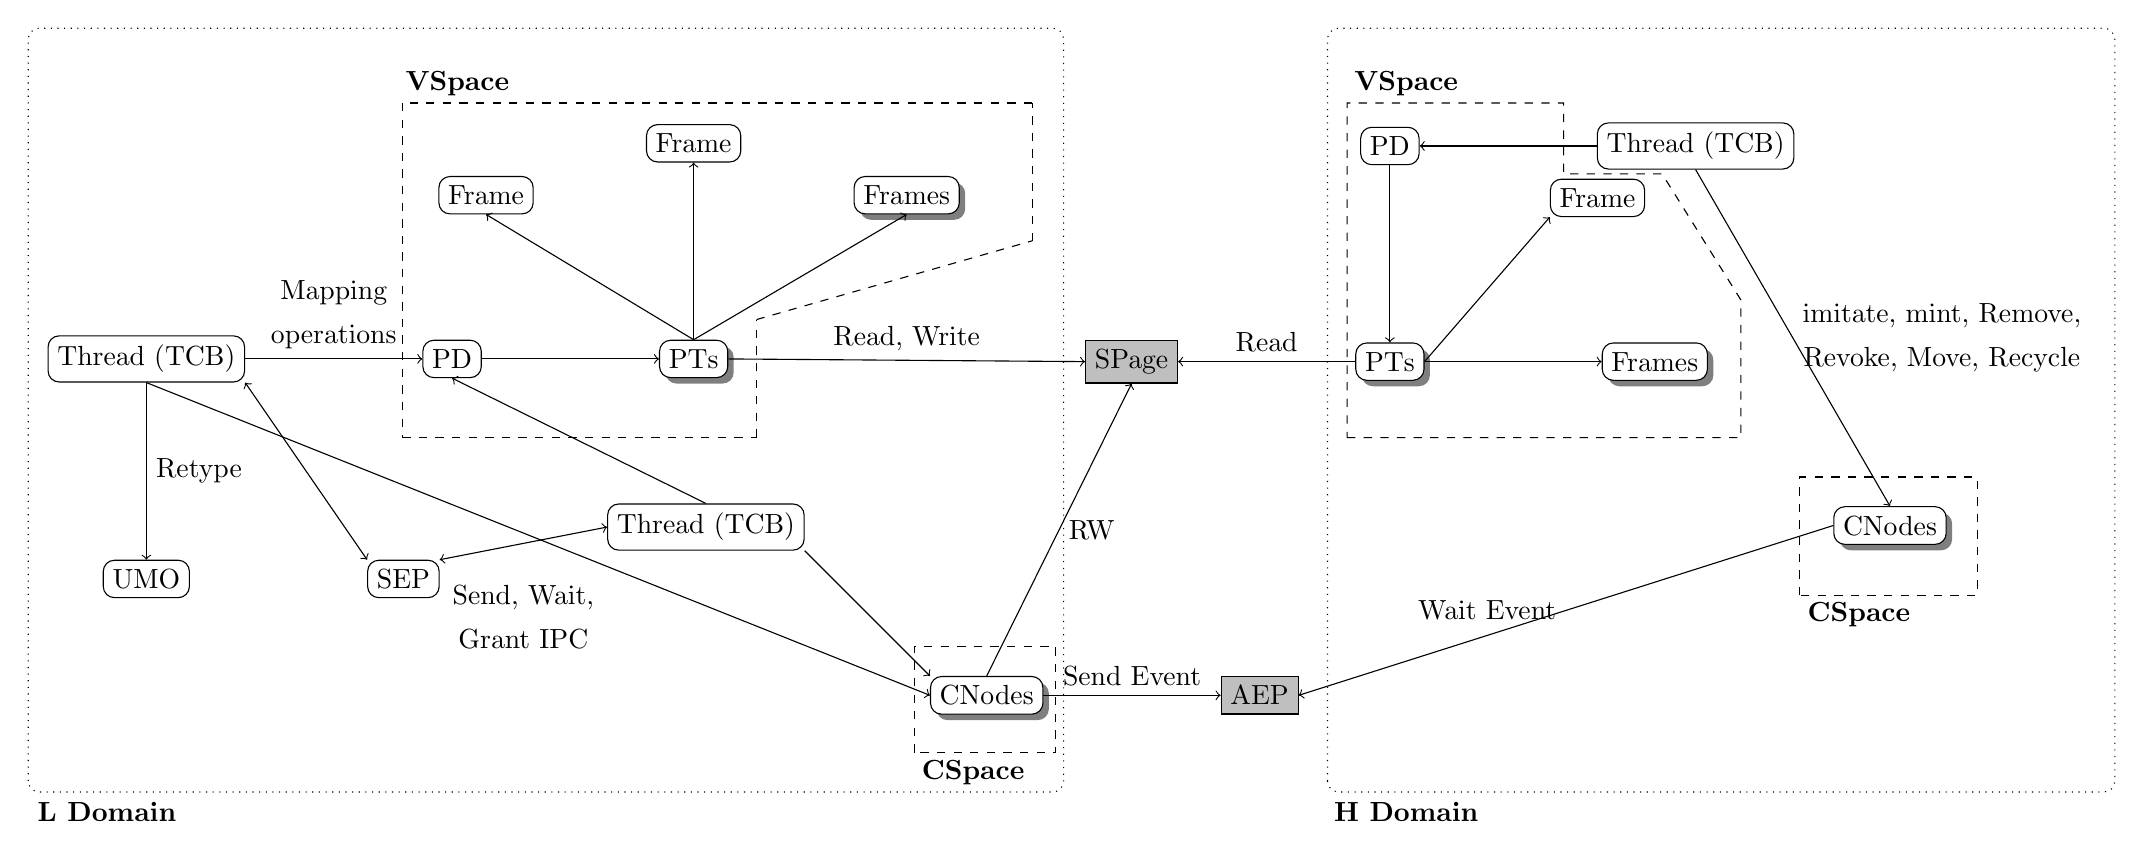
\begin{tikzpicture}[node distance=2.25cm]
\node[draw, rectangle, rounded corners] (T1) {Thread (TCB)};
\node[draw, rectangle, rounded corners] (UMO1)[below=of T1] {UMO};
\draw[->] (T1.south) -- (UMO1.north) node[ midway , right ] {Retype};
\node[draw, rectangle, rounded corners] (PD1) [right=of T1] {PD};
\draw[->] (T1.east) -- (PD1.west)node [above, midway, rectangle split,rectangle split parts=2]{%
  Mapping
  \nodepart{second}
  operations%
  };
\node[draw, rectangle, rounded corners,fill=white, drop shadow={color=black}] (PT1) [right=of PD1] {PTs};
\draw[->] (PD1.east) -- (PT1.west);
\node[draw, rectangle, rounded corners] (P) [above left=of PT1] {Frame};
\node[draw, rectangle, rounded corners] (P2) [above =of PT1] {Frame};
\node[draw, rectangle, rounded corners, fill=white, drop shadow={color=black}] (P3) [above right=of PT1] {Frames};
\draw[->] (PT1.north) -- (P.south);
\draw[->] (PT1.north) -- (P2.south);
\draw[->] (PT1.north) -- (P3.south);
\node[draw, rectangle, rounded corners] (T2) [below right=of PD1] {Thread (TCB)};
\node[draw, rectangle, rounded corners, fill=white, drop shadow={color=black}] (CNode1) [below right=of T2] {CNodes};
\node[draw, rectangle, fill=lightgray] (AEP) [right=of CNode1] {AEP};
\node[draw, rectangle, fill=lightgray] (SP) [below right=of P3] {SPage};
\draw[->] (PT1.east) -- (SP.west) node[midway, above] {Read, Write};
\draw[->] (T2.north) -- (PD1.south);
\node[draw, rectangle, rounded corners] (SEP) [right =of UMO1] {SEP};
\draw[<->] (T2.west) -- (SEP.north east)node [below, midway, rectangle split,rectangle split parts=3]{%
\nodepart{second}
  Send, Wait,
  \nodepart{third}
  Grant IPC%
  };
\draw[<->] (T1.south east) -- (SEP.north west);
\draw[->] (T2.south east) -- (CNode1.north west);
\draw[->] (T1.south) -- (CNode1.west);
\draw[->] (CNode1.north) -- (SP.south) node[ midway , right ] {RW};
\draw[->] (CNode1.east) -- (AEP.west) node[ midway , above ] {Send Event};
\node[draw, rectangle, rounded corners, fill=white, drop shadow={color=black}] (PT2) [right=of SP] {PTs};
\draw[->] (PT2.west) -- (SP.east) node[ midway , above ] {Read};
\node[draw, rectangle, rounded corners] (PD2) [above=of PT2] {PD};
\draw[->] (PD2.south) -- (PT2.north);
\node[draw, rectangle, rounded corners] (T3) [right=of PD2] {Thread (TCB)};
\draw[->] (T3.west) -- (PD2.east);
\node[draw, rectangle, rounded corners] (P4) [above right=of PT2] {Frame};
\node[draw, rectangle, rounded corners, fill=white, drop shadow={color=black}] (P5) [right =of PT2] {Frames};
\draw[->] (PT2.east) -- (P4.south west);
\draw[->] (PT2.east) -- (P5.west);
\node[draw, rectangle, rounded corners, fill=white, drop shadow={color=black}] (CNode2) [below right =of P5] {CNodes};
\draw[->] (T3.south) -- (CNode2.north)node [right, midway, rectangle split,rectangle split parts=2]{%
  imitate, mint, Remove,
  \nodepart{second}
  Revoke, Move, Recycle%
  };
\draw[->] (CNode2.west) -- (AEP.east) node[ midway , above, left ] {Wait Event};
\draw[black, dotted, rounded corners] (-1.5,-5.5) rectangle (11.65,4.2);
\node[font=\bfseries] at (-0.5,-5.75) {L Domain};
\draw[black, dotted, rounded corners] (15,-5.5) rectangle (25,4.2);
\node[font=\bfseries] at (16,-5.75) {H Domain};
\draw[dashed] (3.25,-1) -- (7.75,-1);
\draw[dashed] (7.75,-1) -- (7.75,0.5);
\draw[dashed] (7.75,0.5) -- (11.25,1.5);
\draw[dashed] (11.25,1.5) -- (11.25,3.25);
\draw[dashed] (11.25,3.25) -- (3.25,3.25);
\draw[dashed] (3.25,3.25) -- (3.25,-1);
\node[font=\bfseries] at (3.95,3.5) {VSpace};
\draw[dashed] (15.25,-1) -- (20.25,-1) -- (20.25,0.75) -- (19.25,2.35) -- (18,2.35) -- (18,3.25) -- (15.25,3.25) -- (15.25,-1);
\node[font=\bfseries] at (16,3.5) {VSpace};
\draw[black, dashed] (9.75,-5) rectangle (11.55,-3.65);
\node[font=\bfseries] at (10.5,-5.25) {CSpace};
\draw[black, dashed] (21,-3) rectangle (23.25,-1.5);
\node[font=\bfseries] at (21.75,-3.25) {CSpace};
\end{tikzpicture}
\end{document}